\section{Search regions}
%\minitoc
\subsection{Signal and control region}
Signal region is where it is expected to observe a deviation from SM background in the existence of SUSY scenario. In order to locate this kinematic region a powerful discriminative varible is used. Figure \ref{fig:DF} shows the $\DF$ distribution after the baseline selection. The plot exhbits that the SM background processes peak at zero while the signal models stay flat. Naturally, this shape difference leads to the high values of $\DF$ as the signal region (SR) and the low values as the control region (CR). The control region is used in the background estimation, which will be discussed in the next chapter. It can also be seen from the distribution that after the baseline selection $\wJets$ and $\ttJets$ are the main background components. The $\ttbar$ composition in the CR is dominated by the single leptonic decays while in the SR the di-leptonic  $\ttbar$ decays are dominating. 
 \begin{figure*}[!hbt]
    \begin{center}
 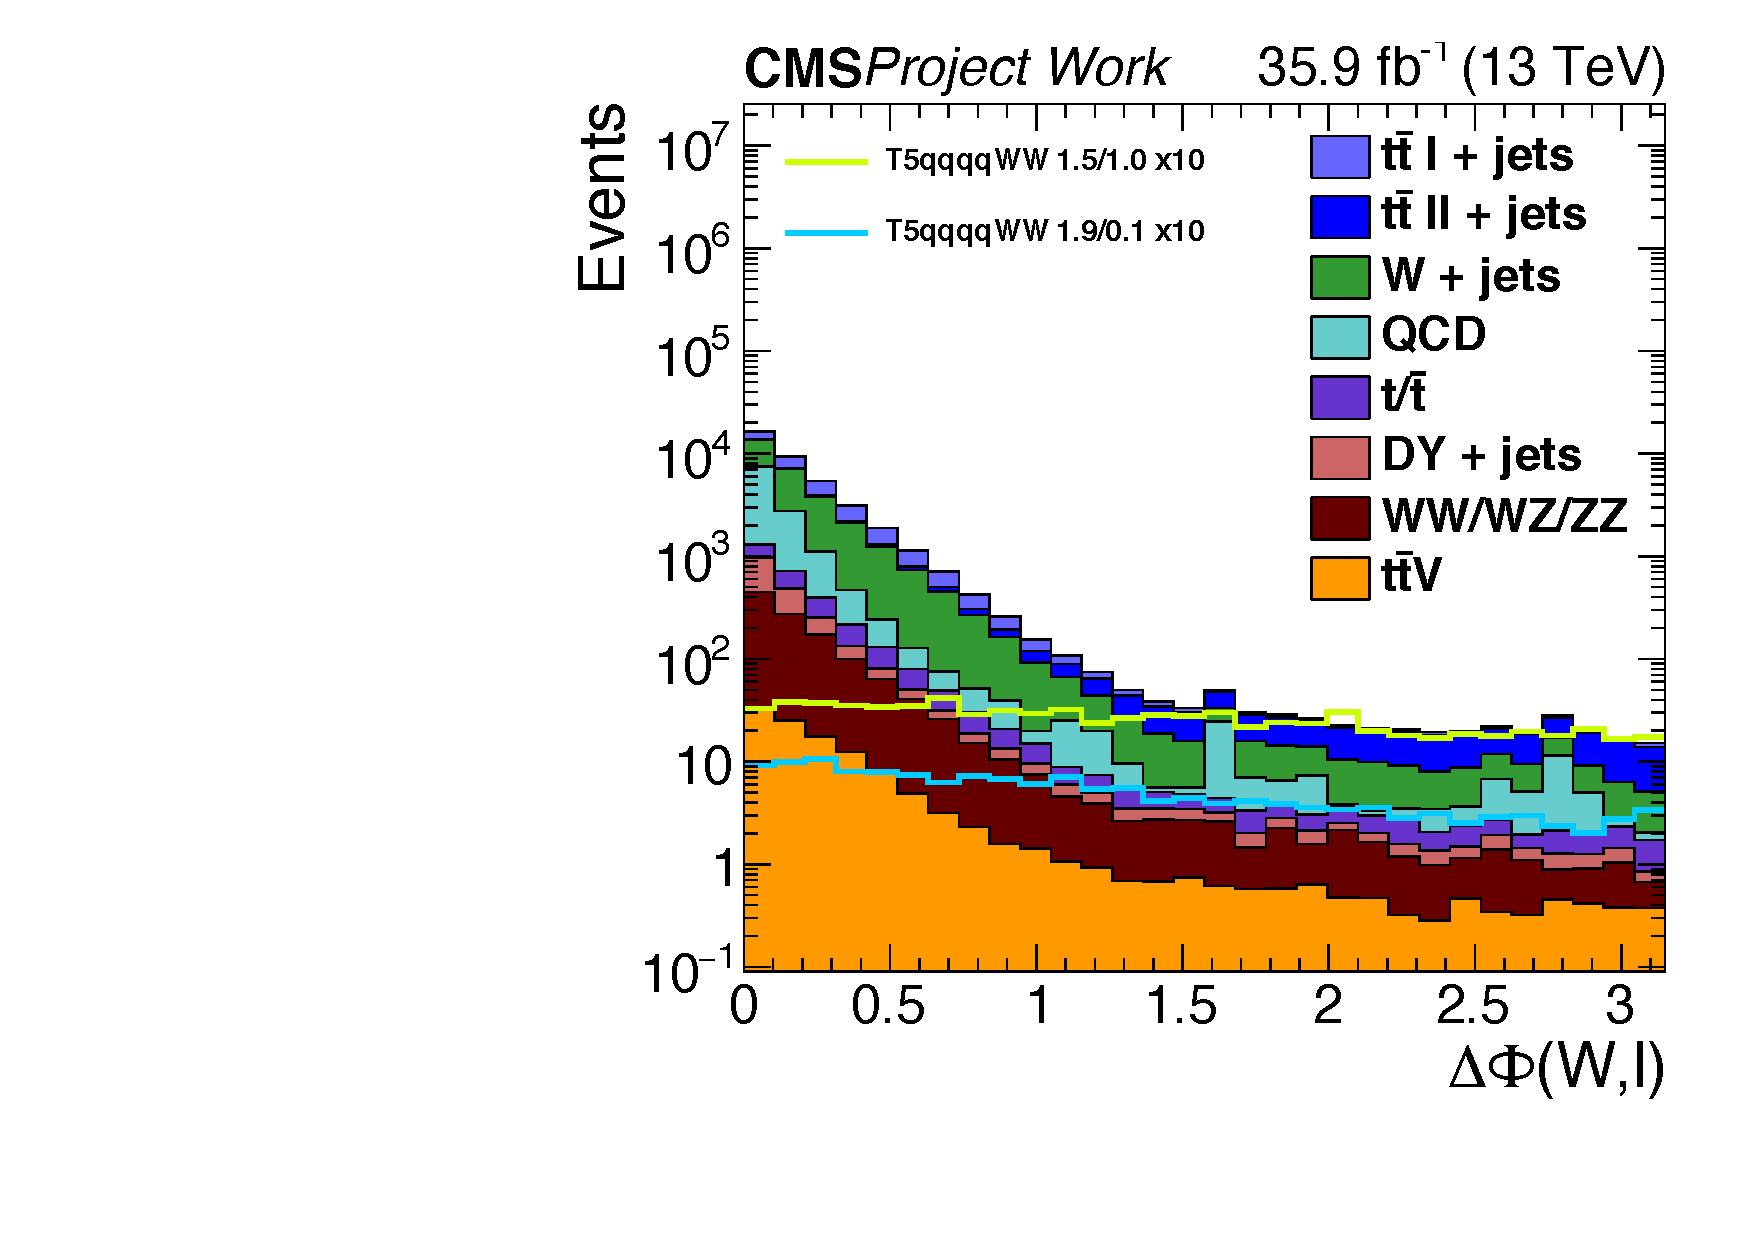
\includegraphics[width=0.5 \textwidth]{Plots/analysis/signalRegions/deltaPhi_Wl_narrownormal}
  \caption{ \label{fig:DF} The $\DF$, after the baseline selection, requiring at least five jets and non of b-tagged, minimum $\HT$ of 500 GeV, a minimum $\LT$ of 250 GeV and exactly one lepton (electron of muon) with $\pt >$25 GeV. The simulated background events are stacked on top of each other, and several signal points are overlaid for illustration without being stacked. The model T5qqqqWW (1.5,1.0) (T5qqqqWW (1.9,0.1)) corresponds to a gluino mass of 1.5 TeV (1.9 TeV) and neutralino mass of 1.1 TeV (0.1 TeV), respectively. The intermediate chargino mass is fixed at 1.25 TeV (1.0 TeV).
  }
   \end{center}
\end{figure*}
\subsection{Main band regions}
To further enhance the sensitivity, the phase space is subdivided in bins of $\njet$, $\HT$ and $\LT$. These sub bins are called main band regions (MB). \\
The binning is designed for an integrated luminosity of 40 fb$^{-1}$ scenario. In the optimization, the bins with the highest figure of merit are chosen among a spectrum of bins. Then, a fully profiled likelihood is performed for the several combinations; The bin combination with the highest sensitivity is chosen. At the same time, for each bin, the yield of background MC is required to be at least one, to have robust background estimation. In addition to these, throughout the bins, boundary cuts are chosen to be symmetric if possible and sensible. For instance, the binning in $\LT$ is same for different $\njet$ bins.\\
The $\DF$ and $\LT$ variables are constructed by using the same objects; $\pt^{lep}$ and $\MET$. Therefore, a correlation can be assumed. As in Figure \ref{fig:2Ds}, for increasing $\LT$ the SM events are located towards the low values of $\DF$. On the other hand, the signal plots do not show the same trend. Therefore, a varying $\DF$  cut, depending on the $\LT$ binning, is used to determine the signal region for each MB. \\
The resultant binning is given in table \ref{tab:signal_regions} and the corresponding simulated background and signal yields can be found in Figures \ref{fig:MCcounts_mu},\ref{fig:MCcounts_ele}. Figures manifest that the di-leptonic decay of $\ttJets$ events are favoured in SR (high $\DF$).
Furthermore, It can also be extracted that simulated QCD multijet events are populated in the CR (low $\DF$) in electron channel.\\
As mentioned, the $\wJets$ and $\ttJets$ are dominating the SM background. In this analysis, the number of the events in the MB SR is estimated with observed data. In the next chapter, the procedure for the estimation of these background components will be explained. \\ 
 \begin{figure*}[!hbt]
    \begin{center}
 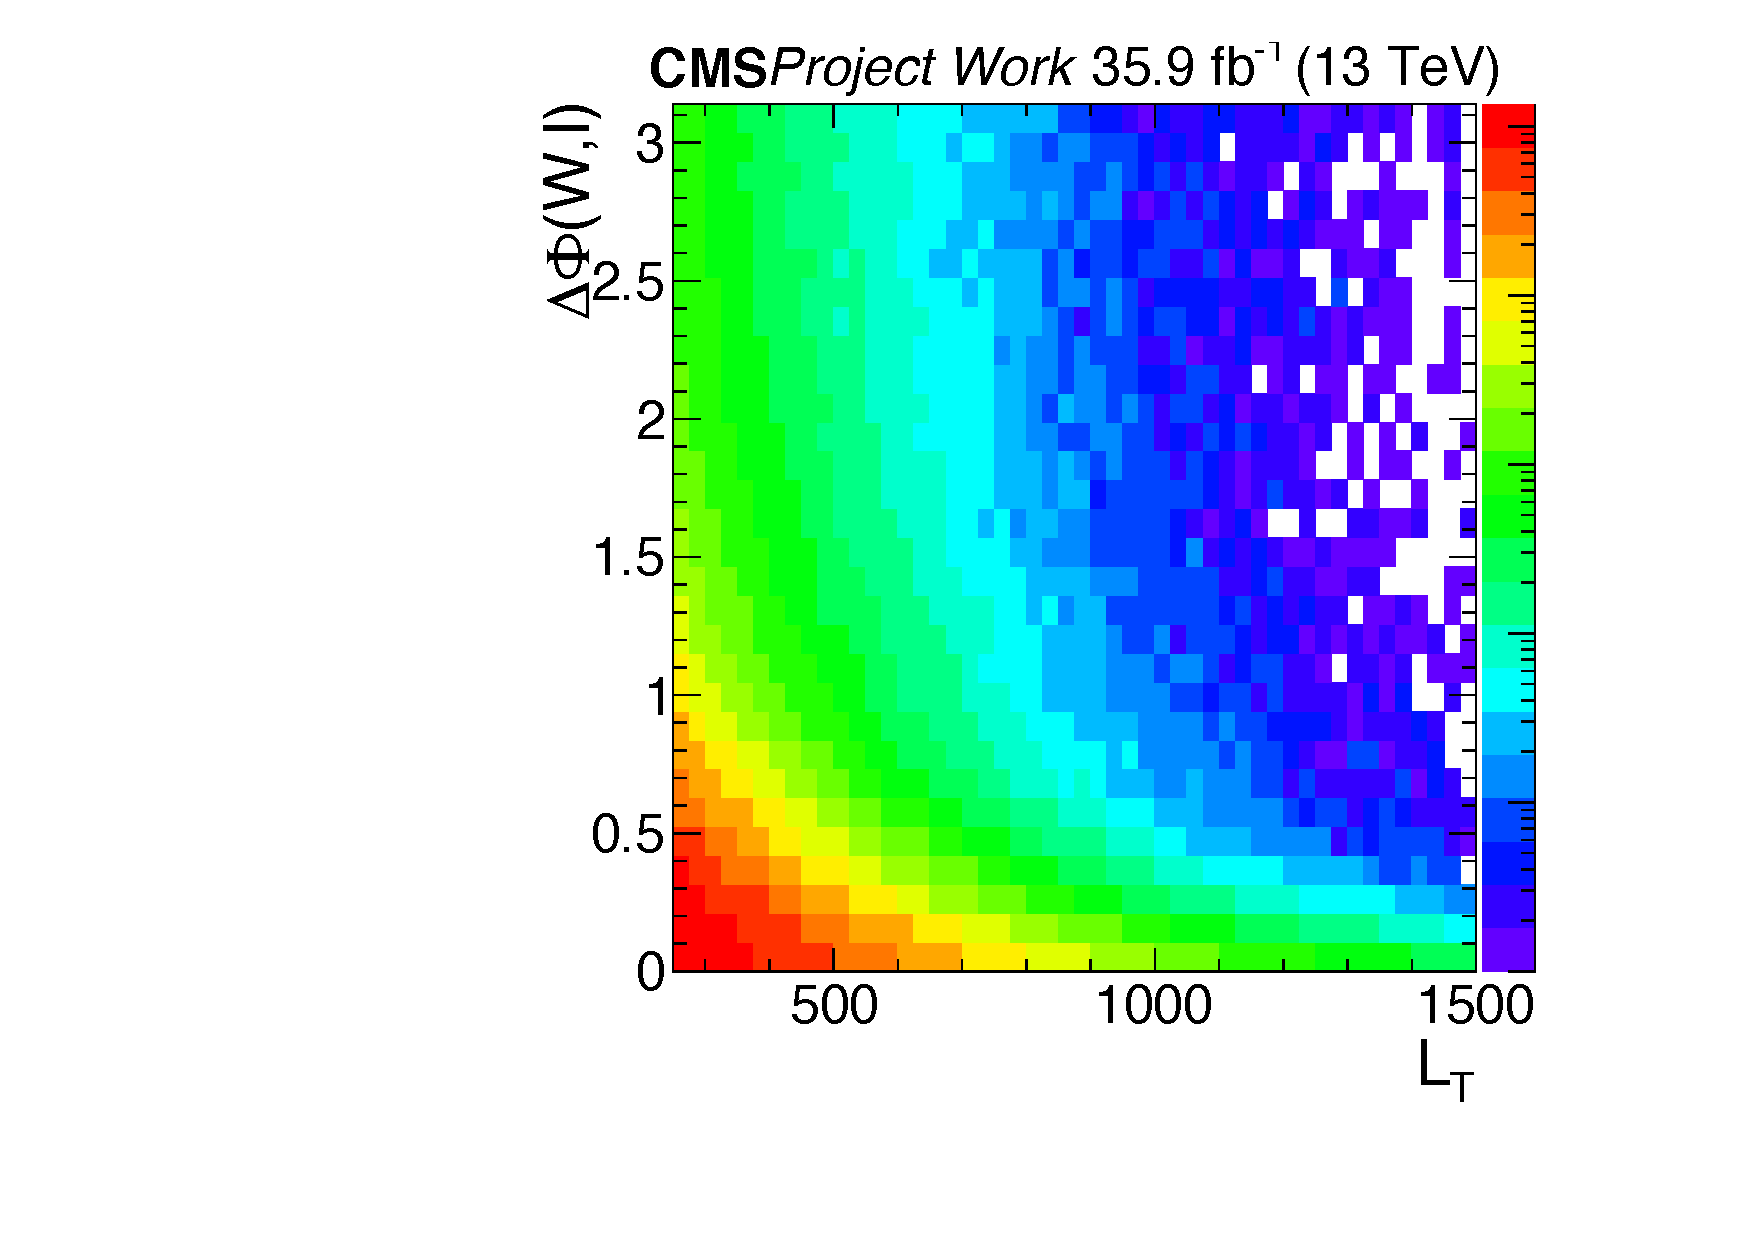
\includegraphics[width=0.45 \textwidth]{Plots/analysis/signalRegions/2D_TTWJets}\\
 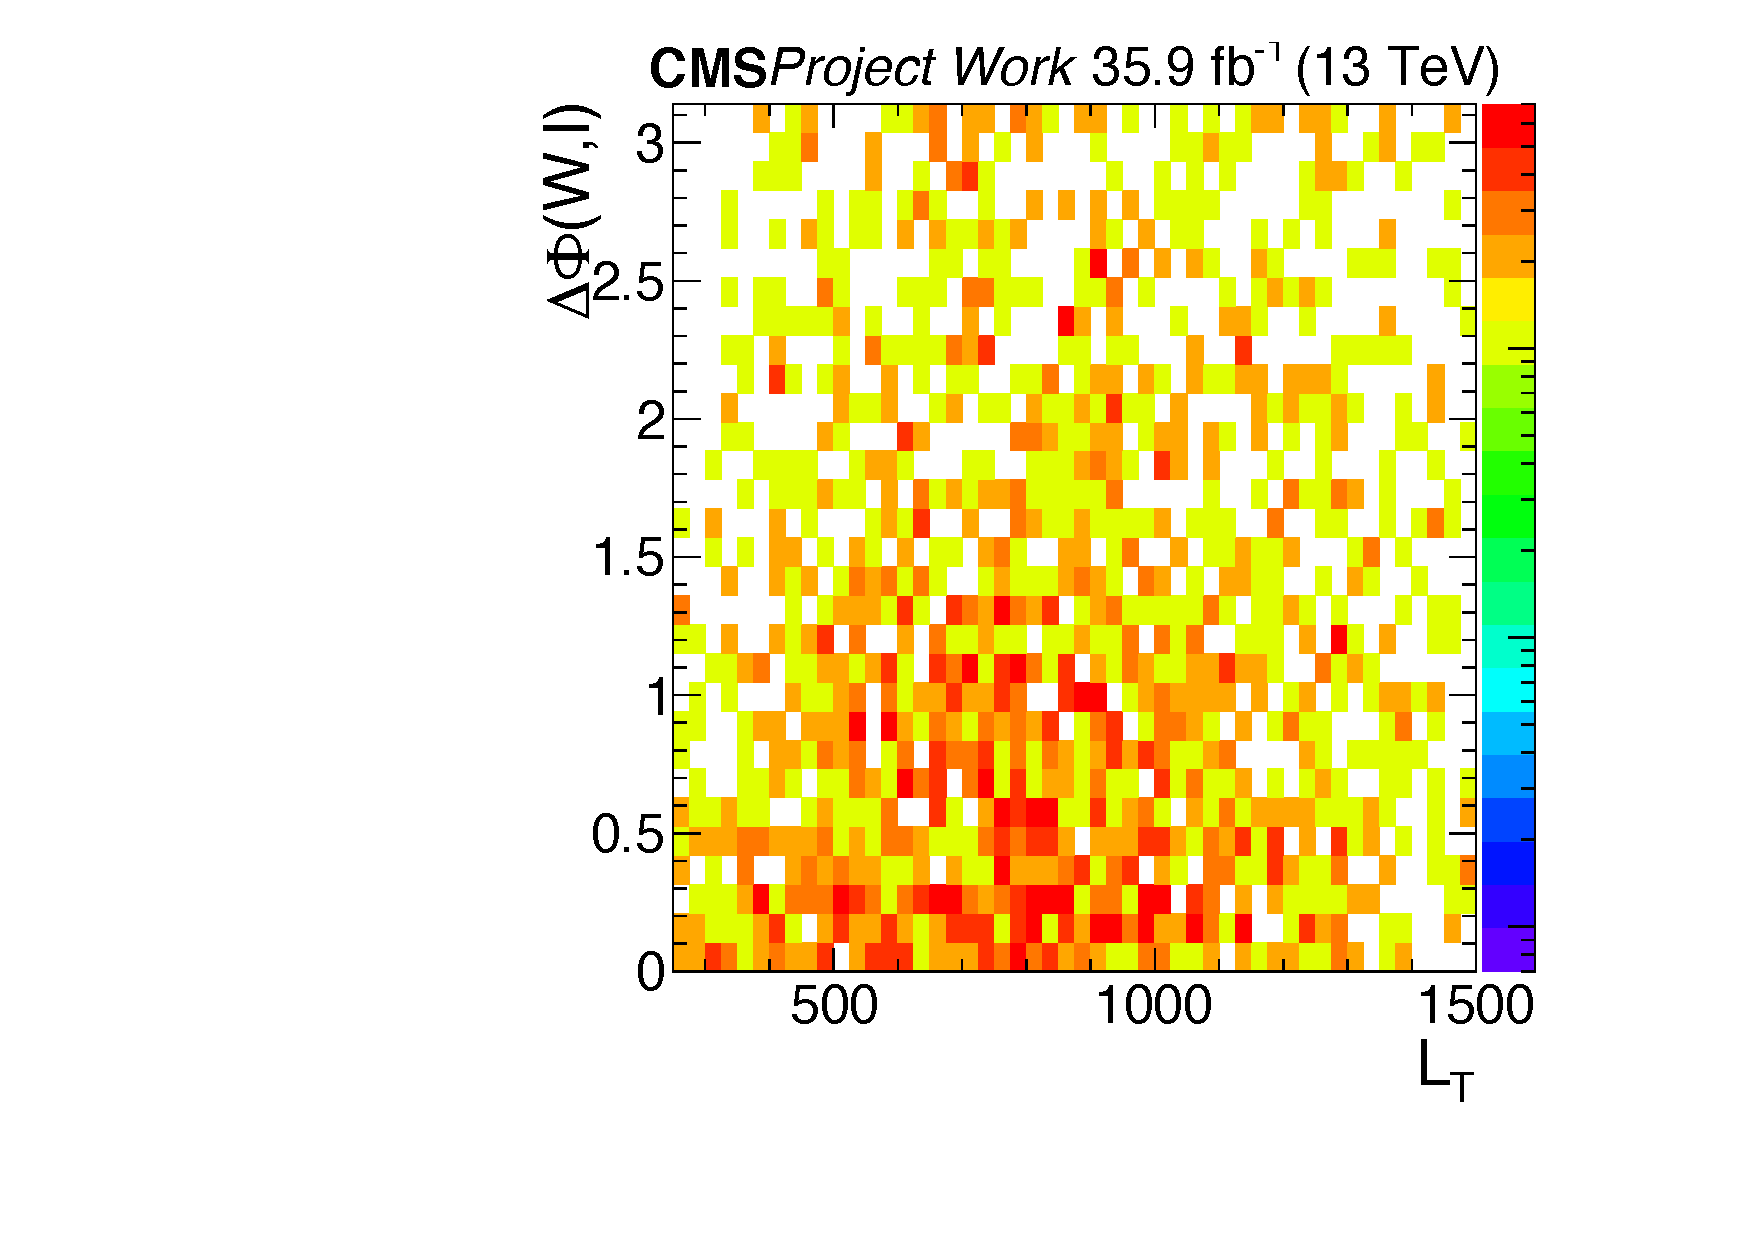
\includegraphics[width=0.45 \textwidth]{Plots/analysis/signalRegions/2D_s1900_100}
 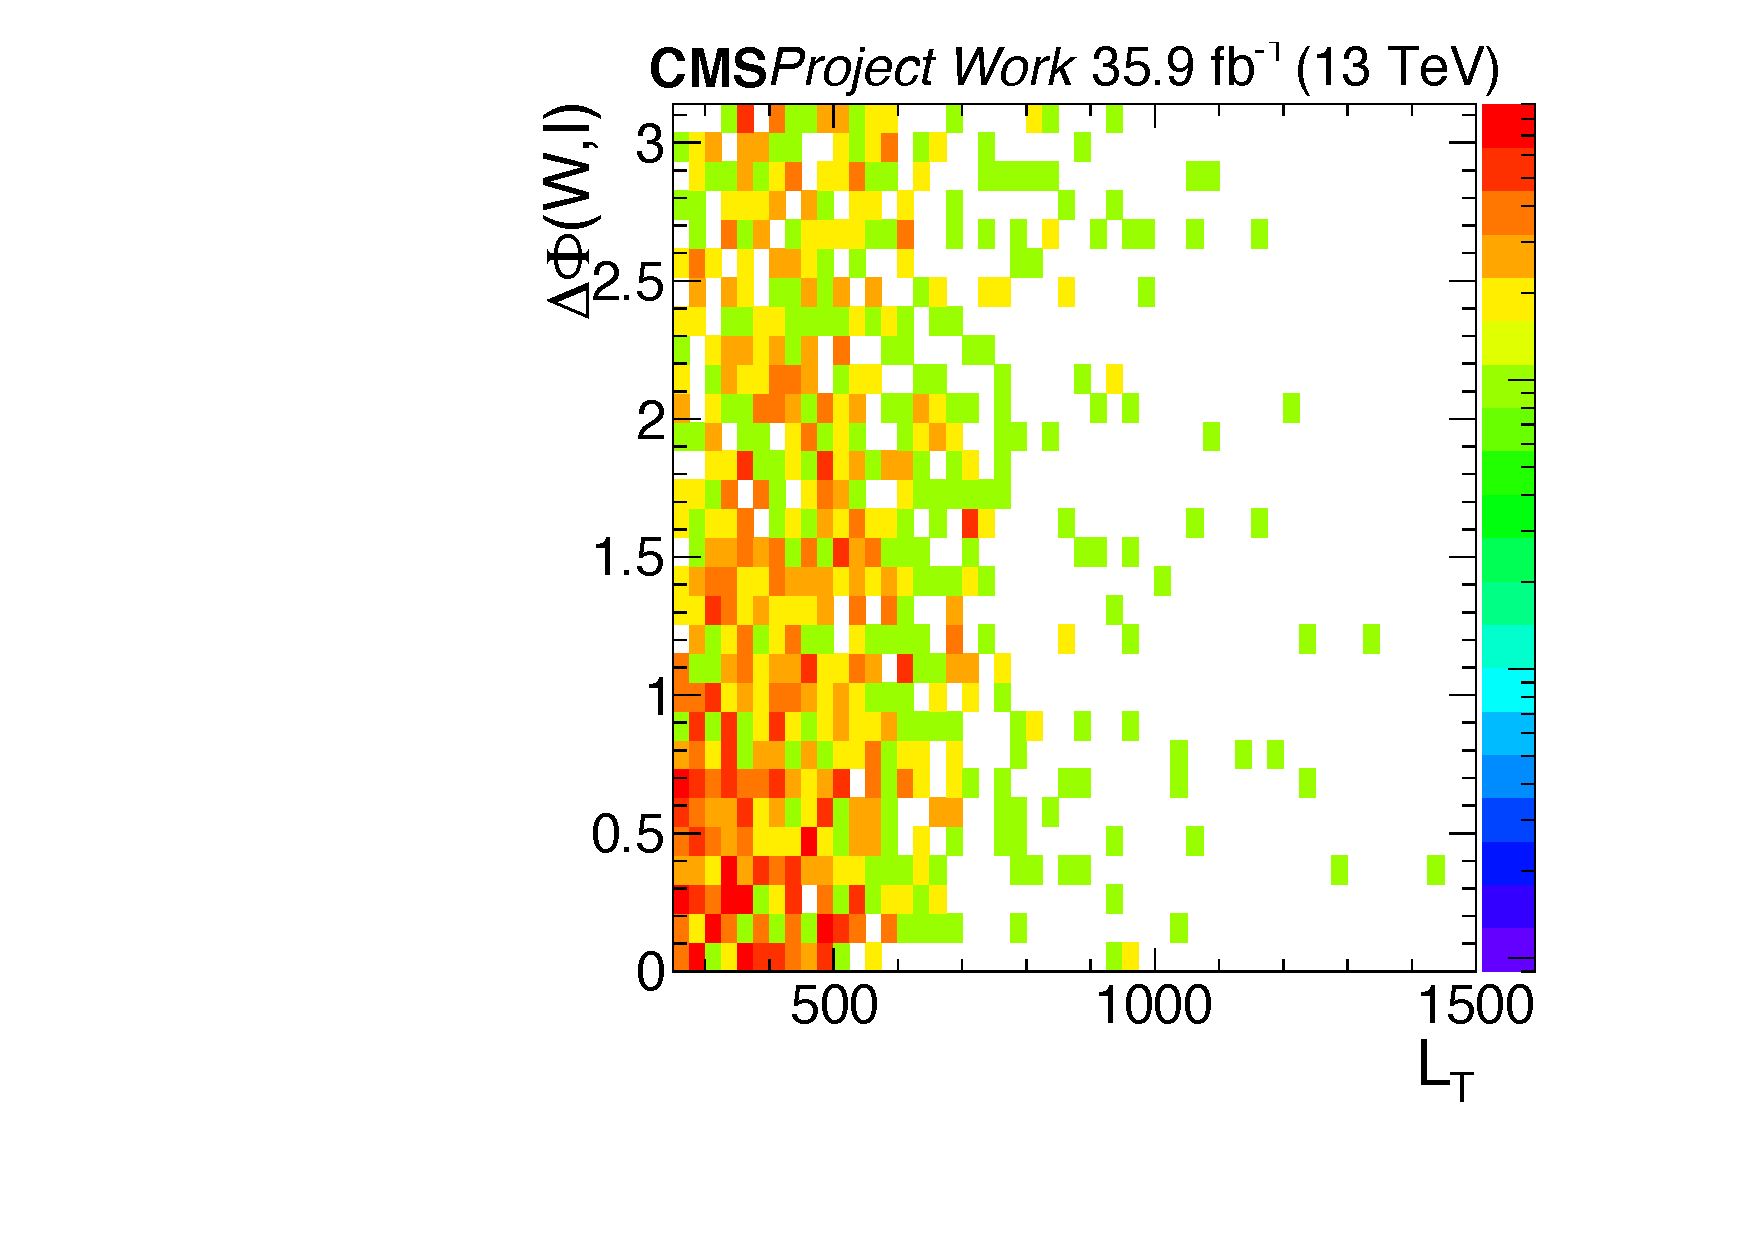
\includegraphics[width=0.45 \textwidth]{Plots/analysis/signalRegions/2D_s1500_1000}
  \caption{ \label{fig:2Ds} 2D distributions of event counts for the main background samples ($\ttJets$ +$\wJets$) (top), and the signal T5qqqWW(1900,100) (left) and T5qqqWW(1500,1000) in the the $\DF$ vs. $\LT$ plane after the preselection.
  }
   \end{center}
\end{figure*}
\\
\textbf{Signal acceptance:}\\
The yield after baseline selection for the simulated signal events is shown in Figure \ref{fig:signalEffs} in the gluino-neutralino mass plane for the T5qqqqWW model. The acceptance of at least one event for 35.9 fb$^{-1}$ integrated luminosity is up to 2250 GeV for gluino mass for the neutralinos masses below 1600 GeV. The equivalent selection efficiency, which is the fraction of baseline events over the total number of simulated events, is presented in the same Figure (top/right).
In the bottom part of Figure, the SR efficiencies are shown. The plot on the left displays the efficiency for the constant $\DF>1$ cut and it is changing between 50-70\%. On the other hand, the left plot shows the efficiency for the variable $\DF$ cut with respect to $\LT$ bin and this time the efficiency goes up to 80\%. 
\begin{figure*}[!hbt]
    \begin{center}
 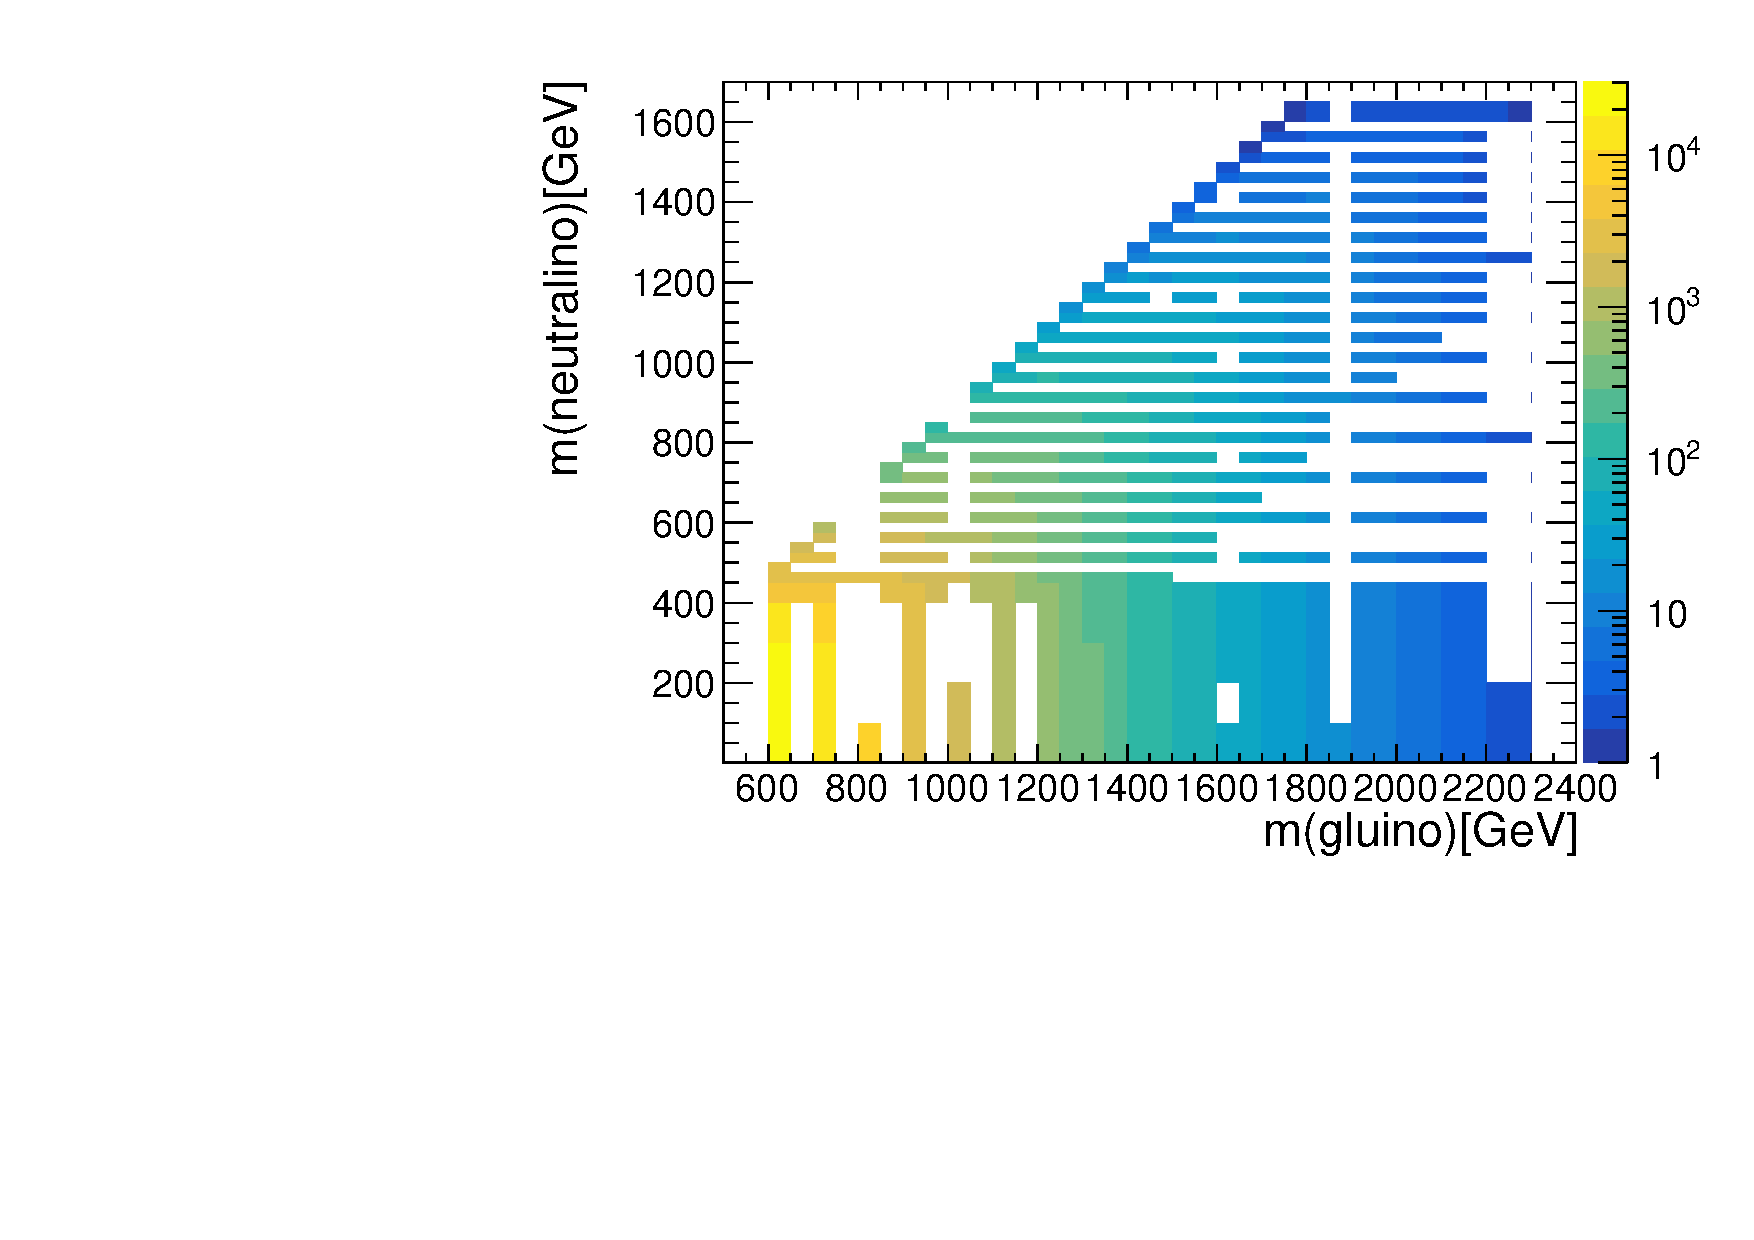
\includegraphics[width=0.45 \textwidth]{Plots/analysis/signalRegions/preselyields}
 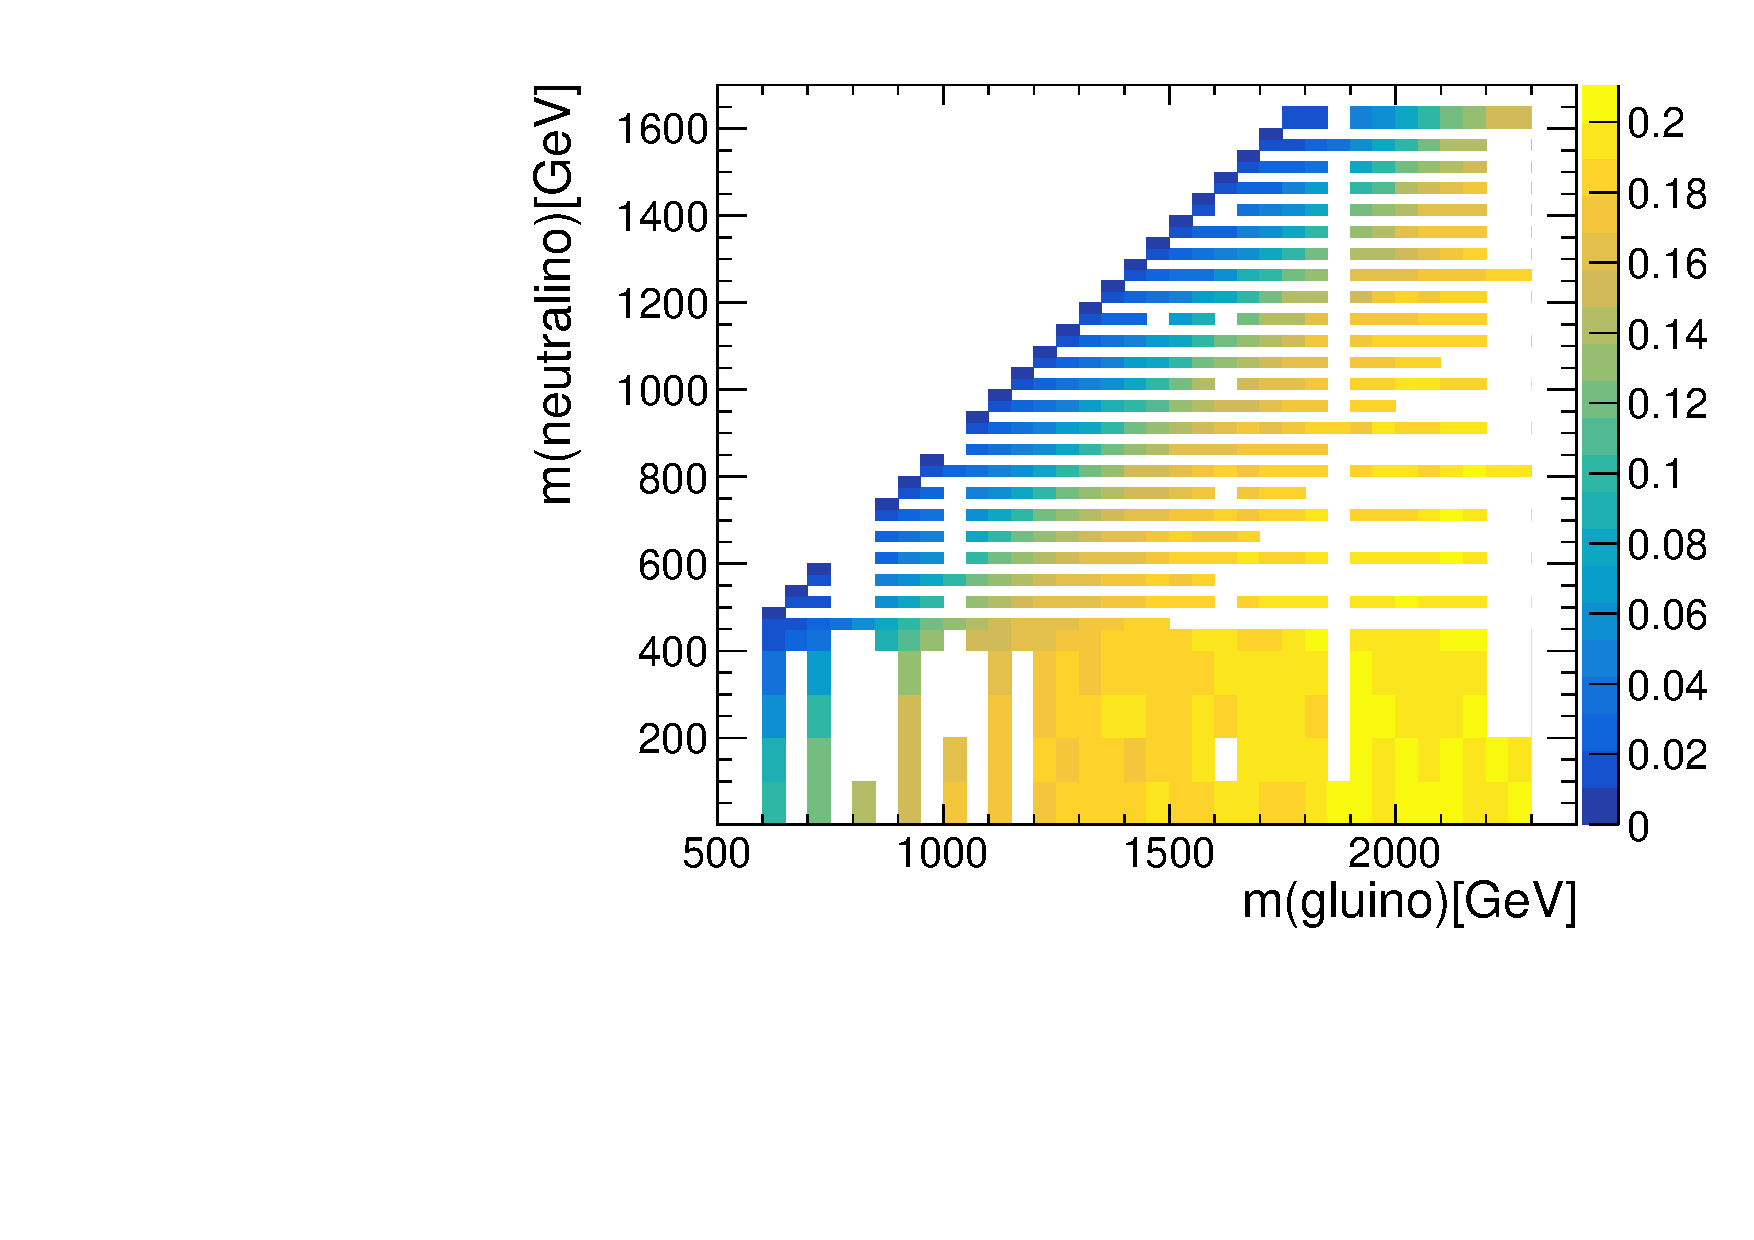
\includegraphics[width=0.4 \textwidth]{Plots/analysis/signalRegions/preselEff}\\
 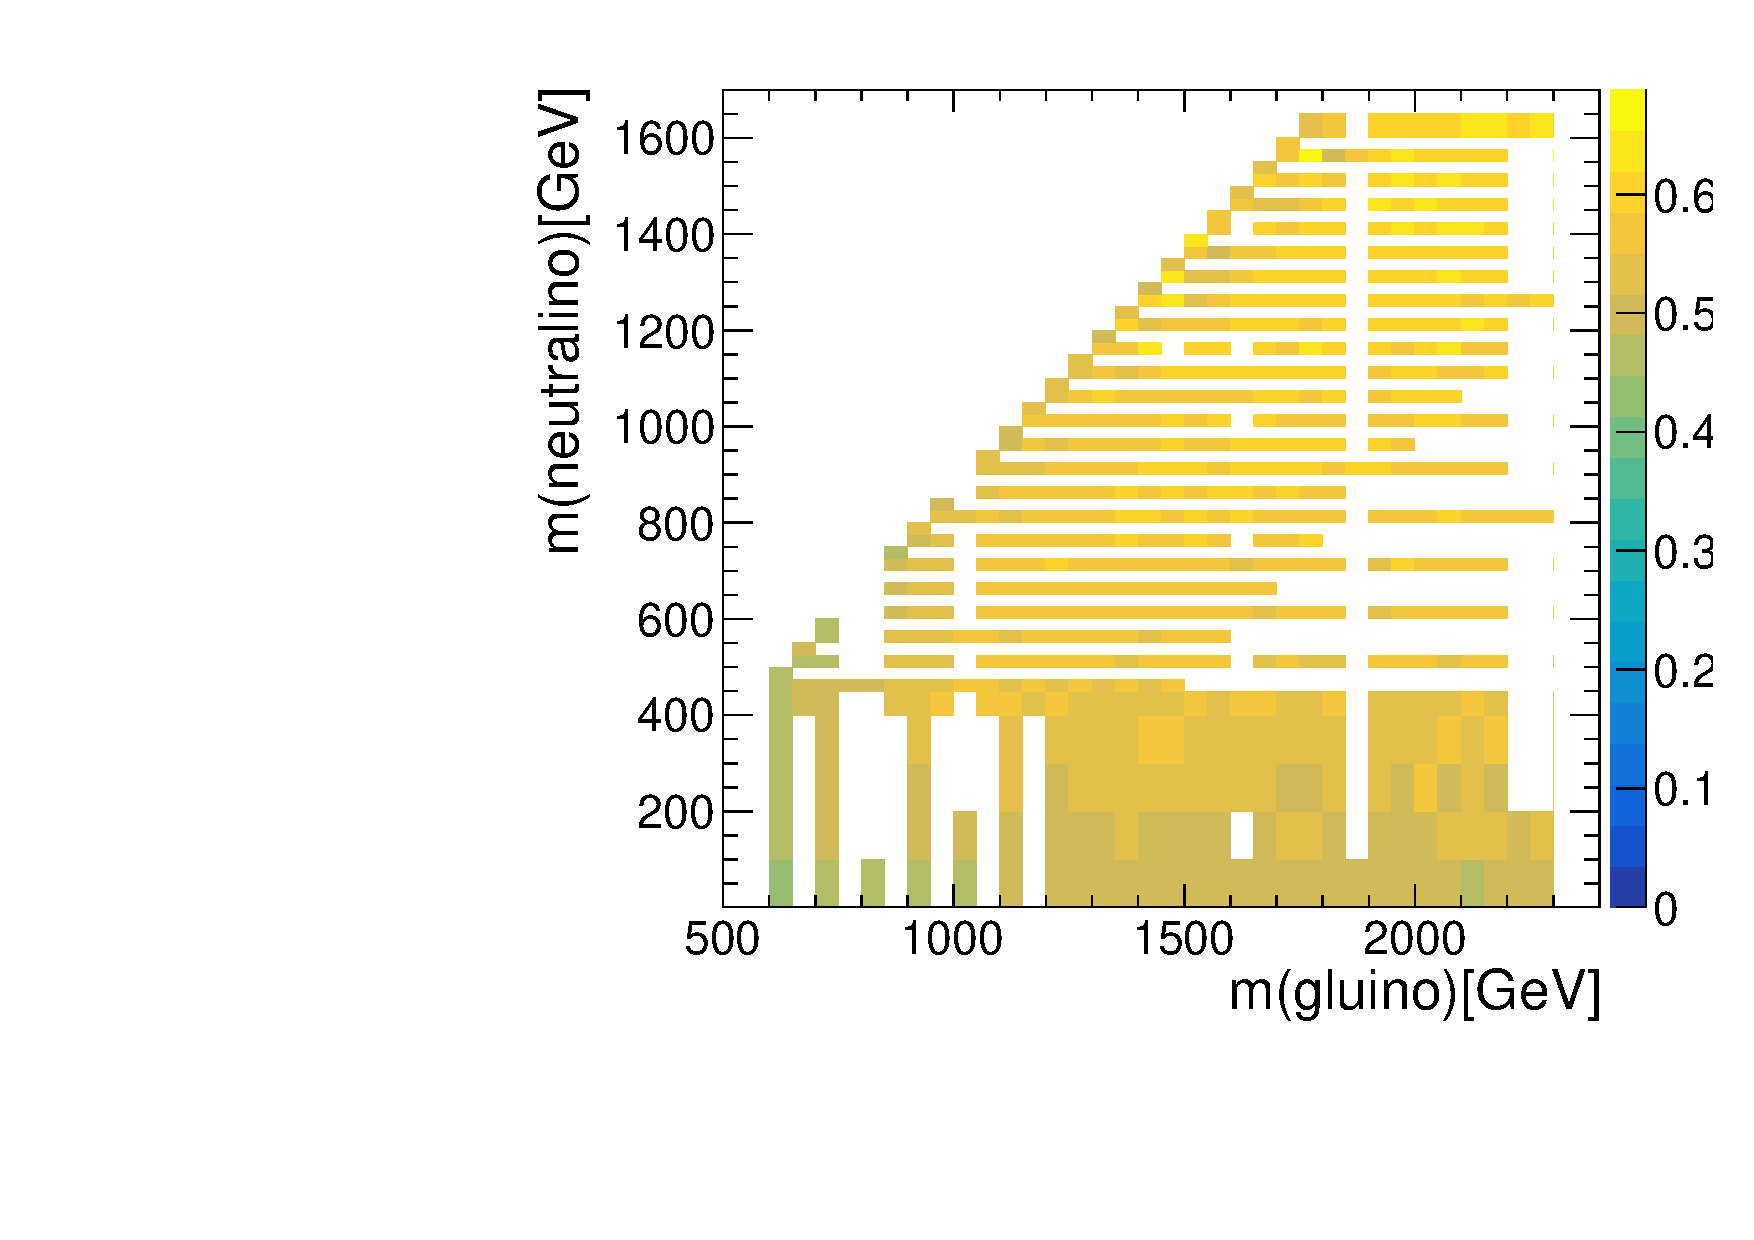
\includegraphics[width=0.4 \textwidth]{Plots/analysis/signalRegions/DF_Eff}
  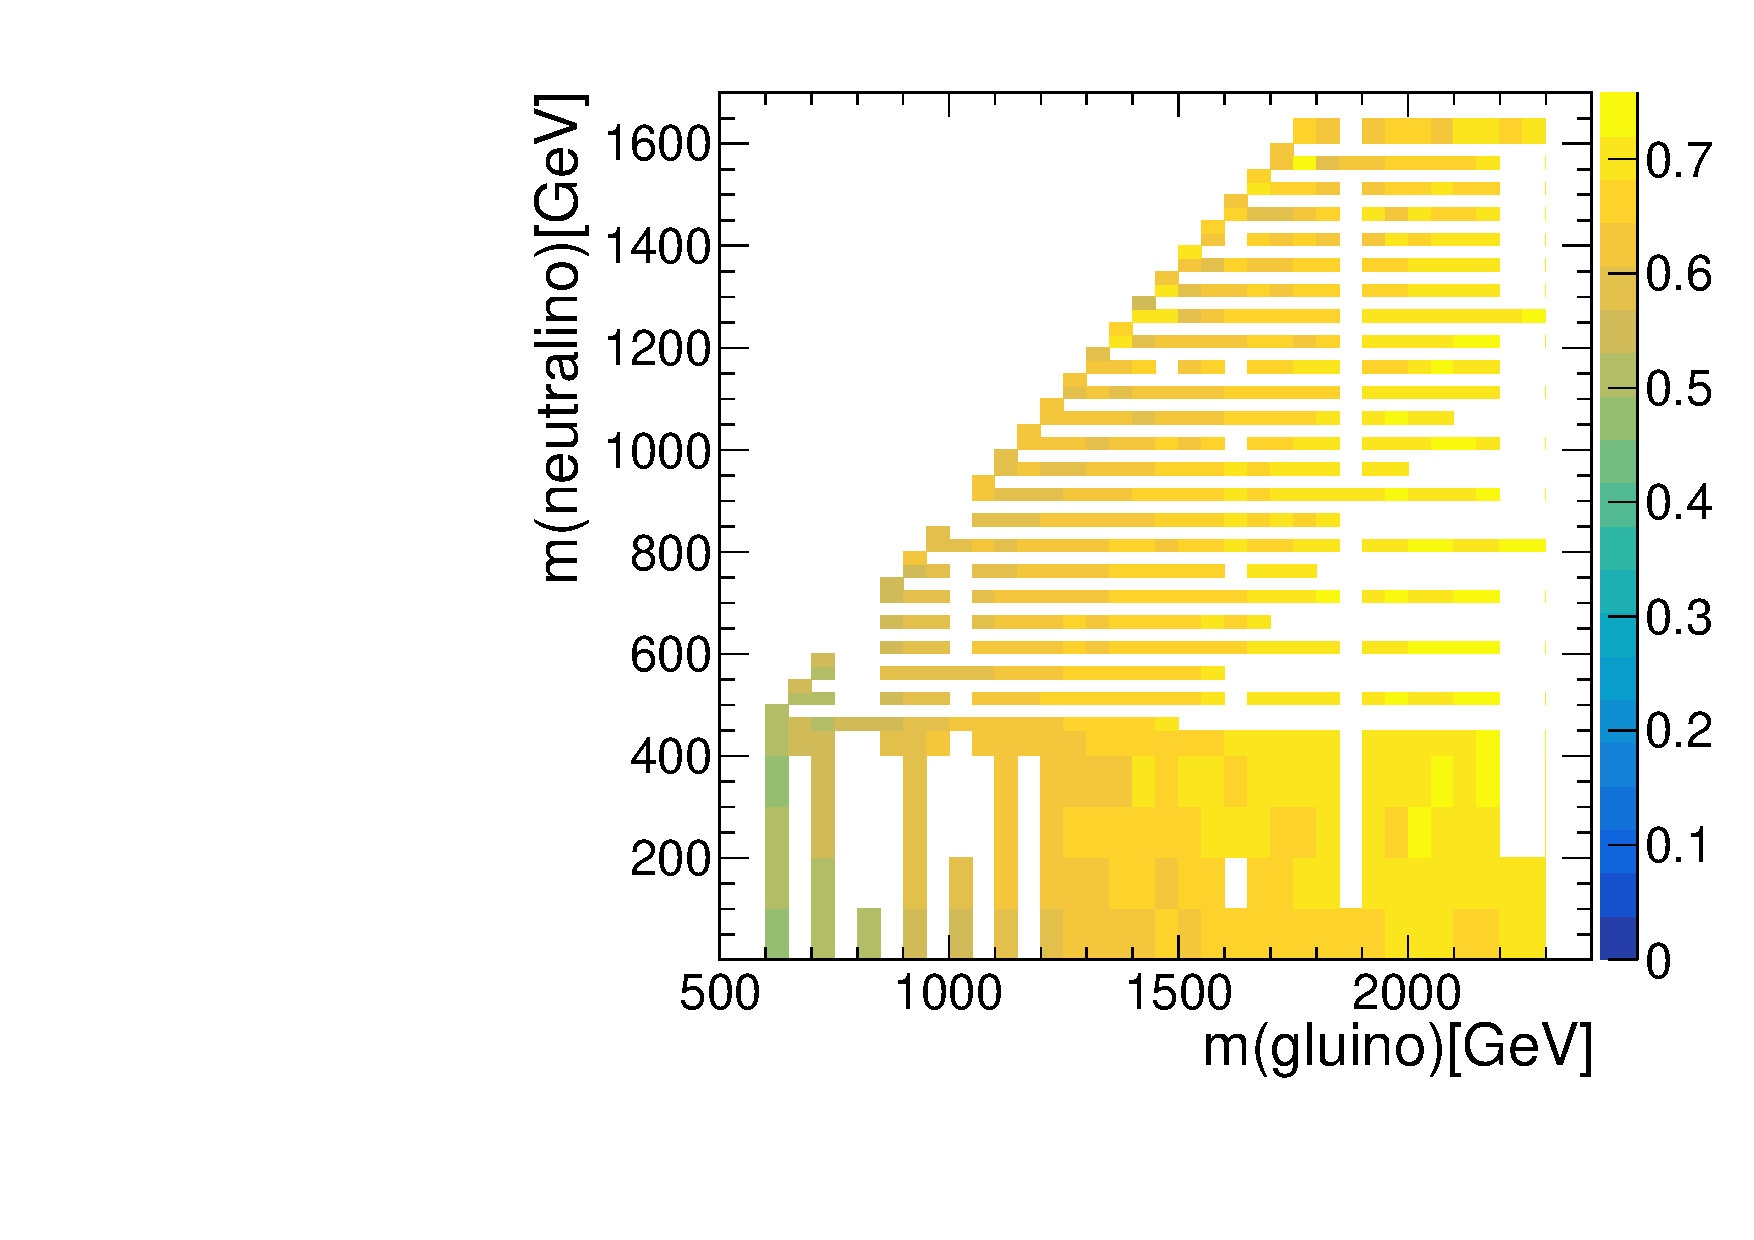
\includegraphics[width=0.4 \textwidth]{Plots/analysis/signalRegions/DF_var_Eff}
  \caption{ \label{fig:signalEffs} The distributions on top represent T5qqqqWW signal counts (left) and selection efficiency (right) after the baseline requirements in the gluino-lsp plane. The distributions at the bottom show the efficiency of signal region selection with respect to the baseline; $\DF>1$ (left) and $\DF>x$ (right) where x stands for the cut value changing according to $\LT$ bin.  
  }
   \end{center}
\end{figure*}
\begin{table}[!htpb]
\begin{center}
\caption{Signal regions.}
\label{tab:signal_regions}
\begin{tabular}{c|c|c}\hline\hline
\multicolumn{3}{c}{5 jets, 0 b-tagged jets}\\\hline
\LT$[$GeV$]$ & \HT$[$GeV$]$ & \DF \\\hline
\multirow{2}{*}{$[250,350]$} & $[500,750]$ & 1.0\\
 & $\geq750$ & 1.0\\\hline
\multirow{2}{*}{$[350,450]$} & $[500,750]$ & 1.0\\
 & $\geq750$ & 1.0\\\hline
\multirow{3}{*}{$[450,650]$} & $[500,750]$ & 0.75\\
 & $[750,1250]$ & 0.75\\
 & $\geq1250$ & 0.75\\\hline
\multirow{3}{*}{$\geq650$} & $[500,750]$ & 0.50\\
 & $[750,1250]$ & 0.50\\
 & $\geq1250$ & 0.50\\\hline\hline
\multicolumn{3}{c}{$[6$,$7]$ jets, 0 b-tagged jets}\\\hline
\LT$[$GeV$]$ & \HT$[$GeV$]$ & \DF \\\hline
\multirow{2}{*}{$[250,350]$} & $[500,1000]$ & 1.0\\
 & $\geq1000$ & 1.0\\\hline
\multirow{2}{*}{$[350,450]$} & $[500,1000]$ & 1.0\\
 & $\geq1000$ & 1.0\\\hline
\multirow{3}{*}{$[450,650]$} & $[500,750]$ & 0.75\\
 & $[750,1250]$ & 0.75\\
 & $\geq1250$ & 0.75\\\hline
\multirow{3}{*}{$\geq650$} & $[500,750]$ & 0.50\\
 & $[750,1250]$ & 0.50\\
 & $\geq1250$ & 0.50\\\hline\hline
\multicolumn{3}{c}{$\geq 8$ jets, 0 b-tagged jets}\\\hline
\LT$[$GeV$]$ & \HT$[$GeV$]$ & \DF \\\hline
\multirow{2}{*}{$[250,350]$} & $[500,1000]$ & 1.0\\
 & $\geq1000$ & 1.0\\\hline
\multirow{2}{*}{$[350,450]$} & $[500,1000]$ & 1.0\\
 & $\geq1000$ & 1.0\\\hline
\multirow{2}{*}{$[450,650]$} & $[500,1250]$ & 0.75\\
 & $\geq1250$ & 0.75\\\hline
\multirow{2}{*}{$\geq650$} & $[500,1250]$ & 0.50\\
 & $\geq1250$ & 0.50\\\hline\hline
\hline
\end{tabular}
\end{center}
\end{table}

 \begin{figure*}[!hbt]
    \begin{center}
 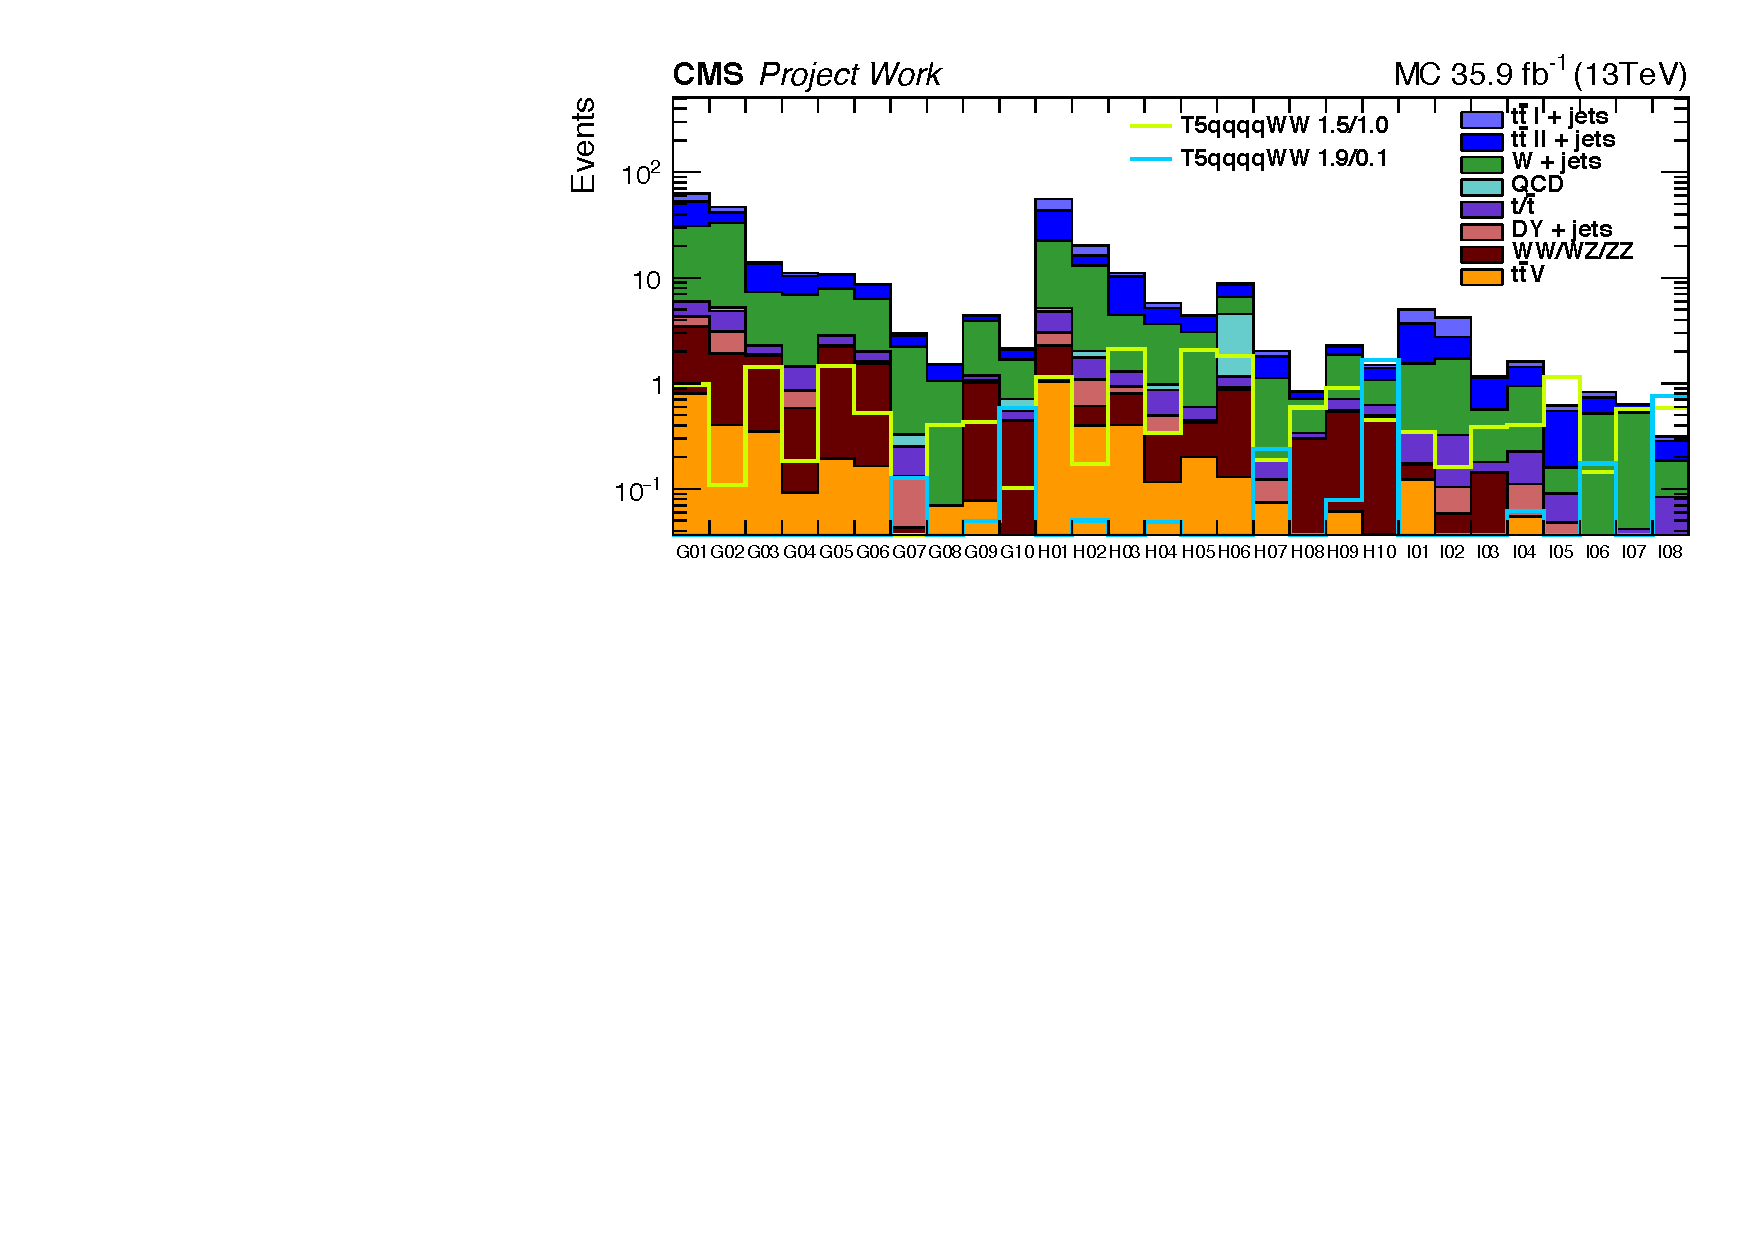
\includegraphics[width=0.95 \textwidth]{Plots/analysis/signalRegions/MC__mu__SR}\\
   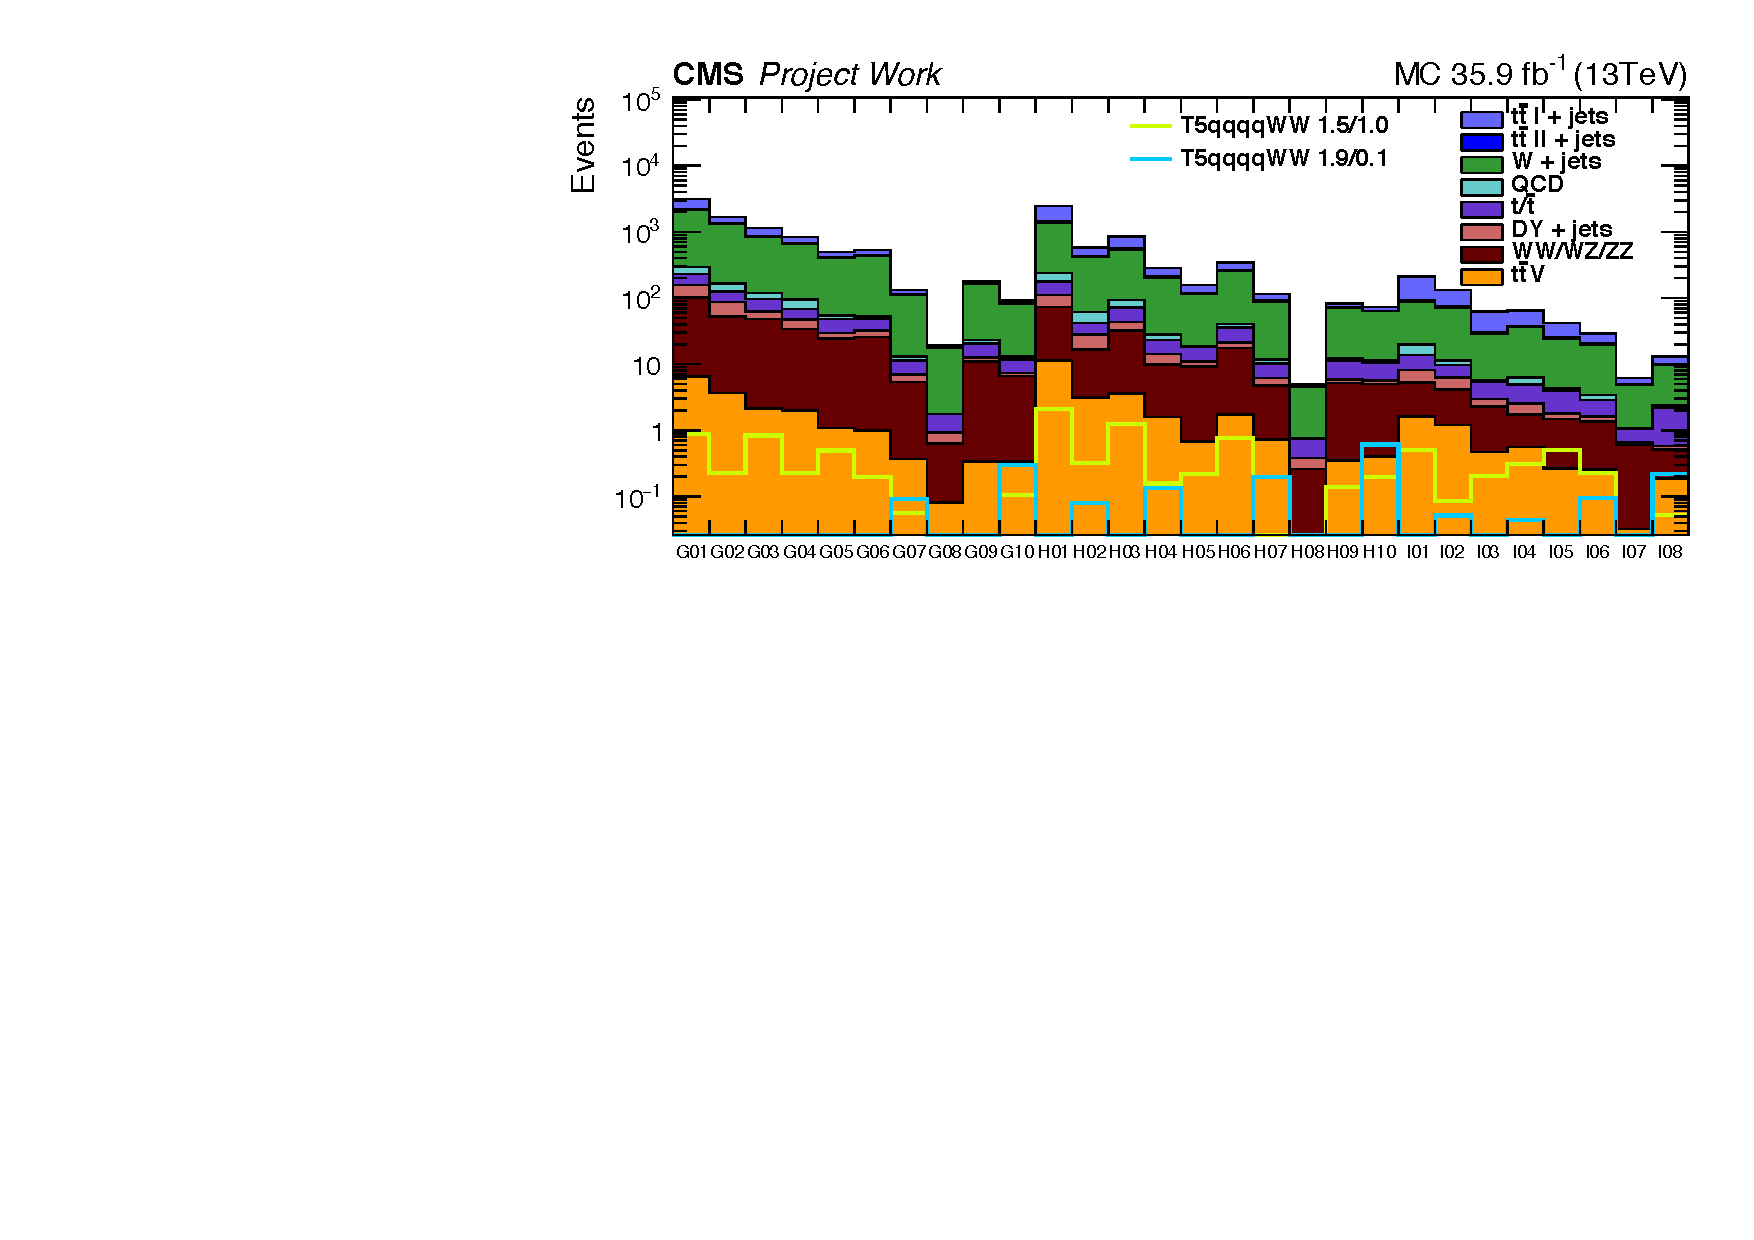
\includegraphics[width=0.95 \textwidth]{Plots/analysis/signalRegions/MC__mu__CR}
  \caption{ \label{fig:MCcounts_mu} Simulated single muon event yields for the background processes are shown as color filled stacked histograms for all 28 search bins. The two signal benchmark models are overlayed and shown by line histograms. The upper plot shows the high $\DF$ regions (SR) while the lower plot shows the low $\DF$ regions (CR).
  }
   \end{center}
\end{figure*}

 \begin{figure*}[!hbt]
    \begin{center}
 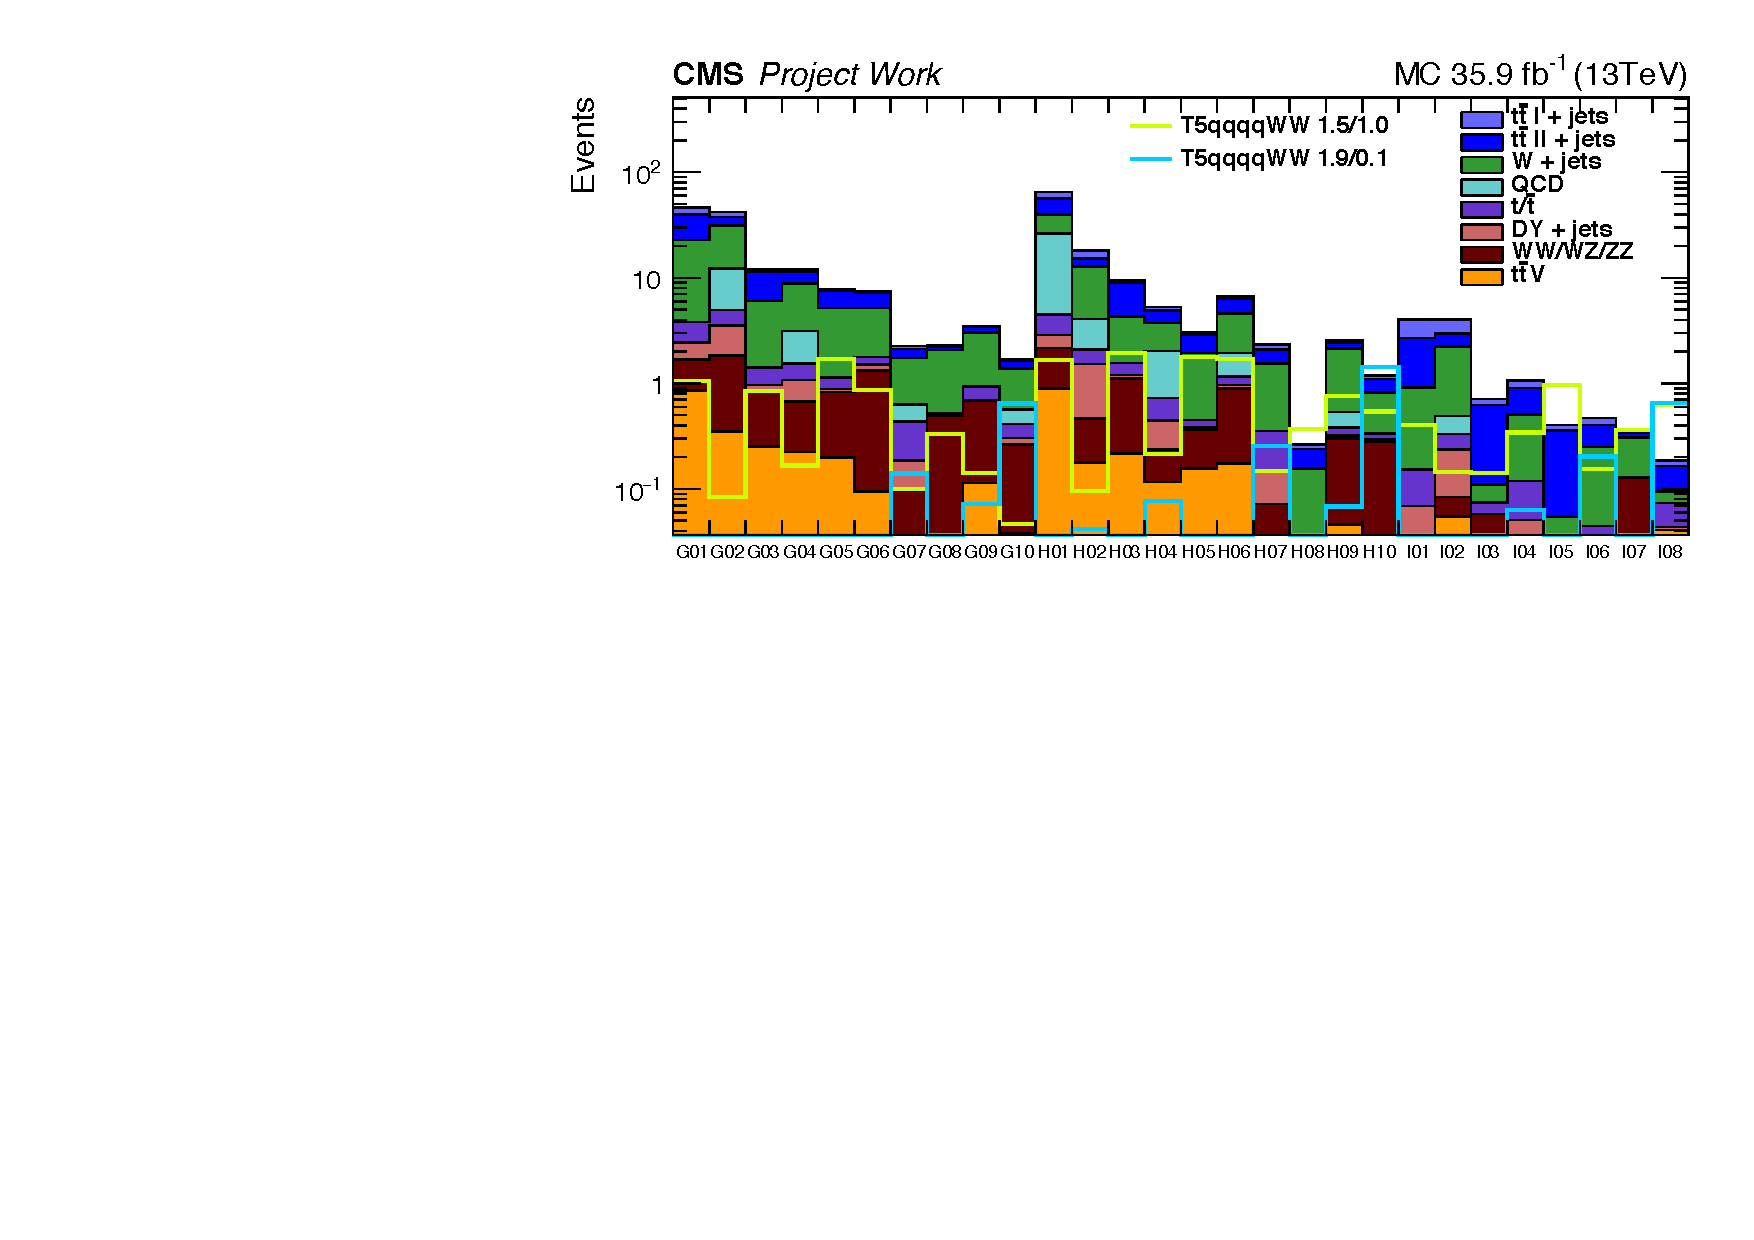
\includegraphics[width=0.95 \textwidth]{Plots/analysis/signalRegions/MC__ele__SR}\\
   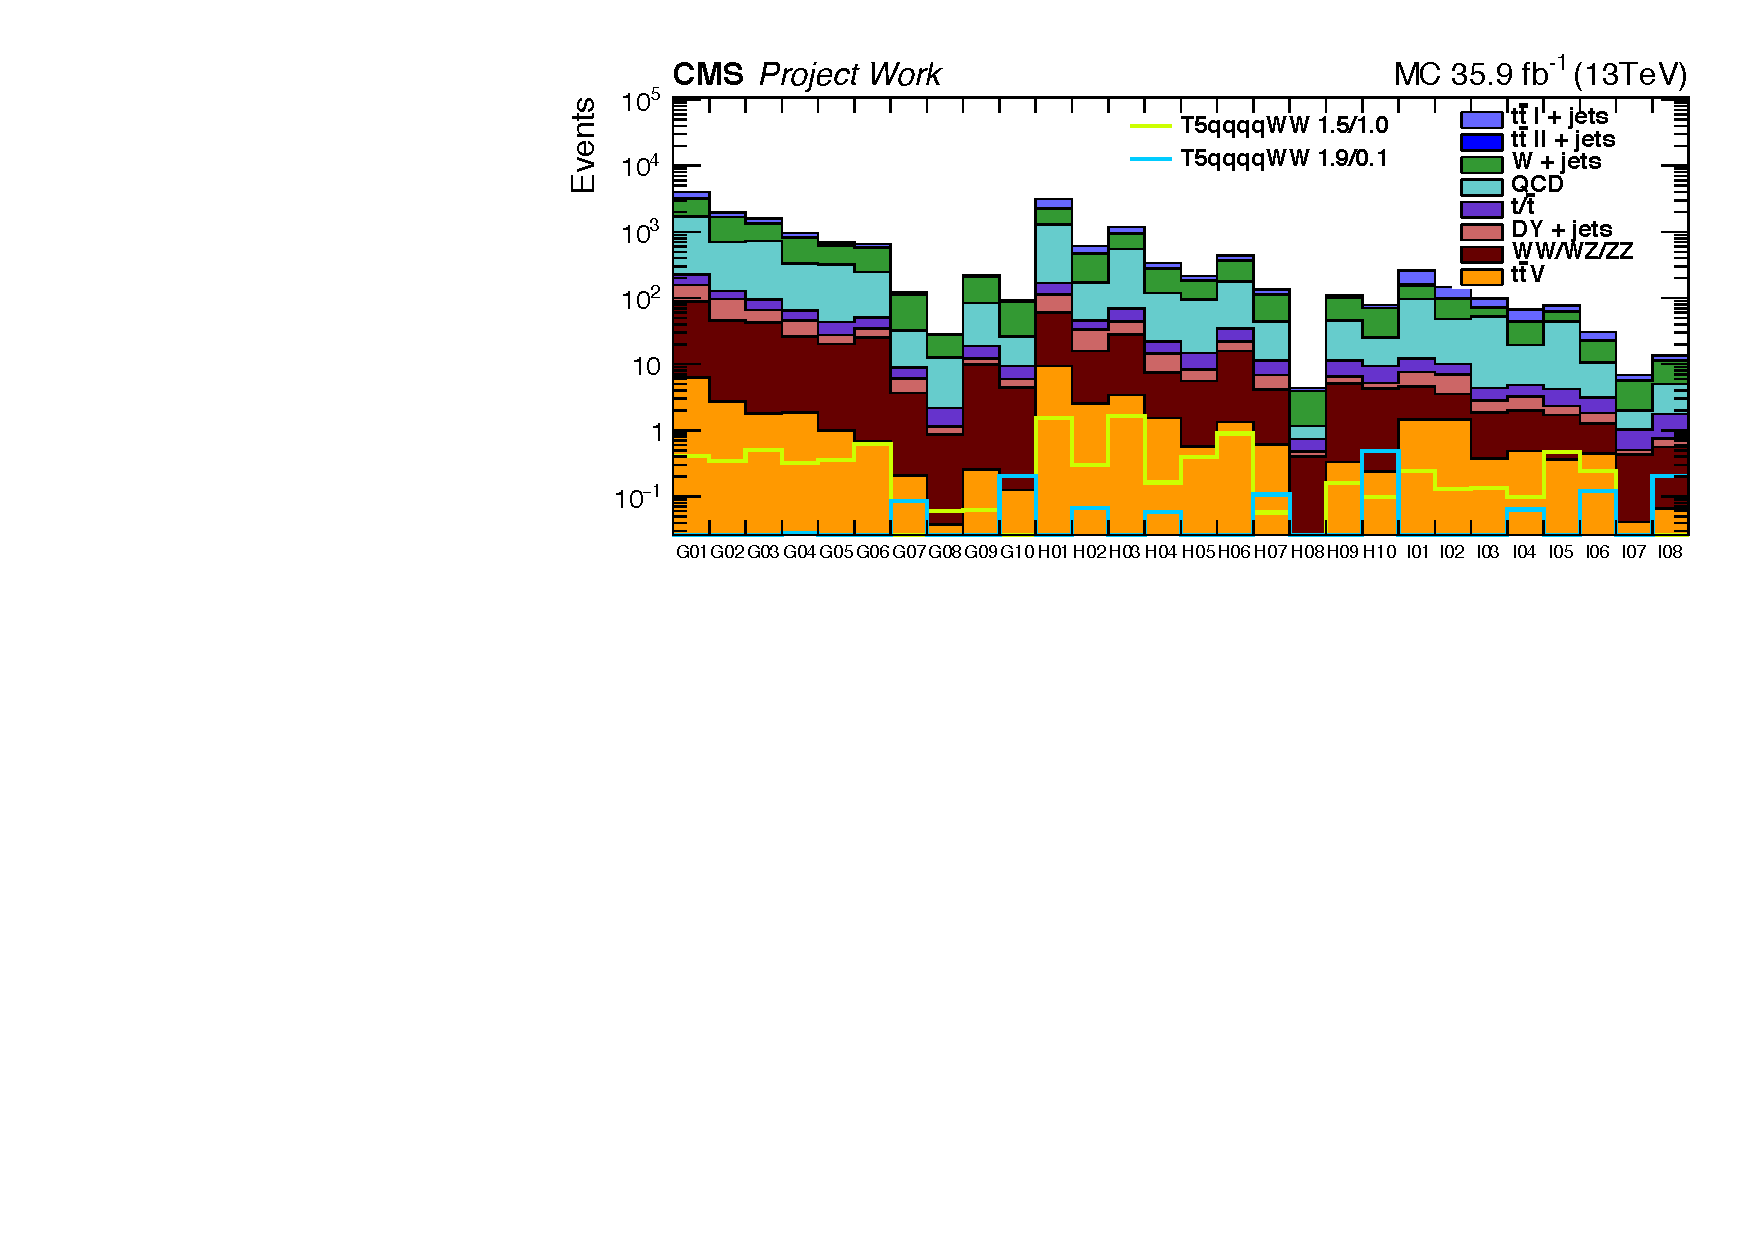
\includegraphics[width=0.95 \textwidth]{Plots/analysis/signalRegions/MC__ele__CR}
  \caption{ \label{fig:MCcounts_ele} Simulated single electron event yields for the background processes are shown as color filled stacked histograms for all 28 search bins. The two signal benchmark models are overlayed and shown by line histograms. The upper plot shows the high $\DF$ regions (SR) while the lower plot shows the low $\DF$ regions (CR).
  }
   \end{center}
\end{figure*}